A beam of light strikes $\overline{BC}$ at point $C$ with angle of incidence $\alpha=19.94^\circ$ and reflects with an equal angle of reflection as shown.  The light beam continues its path, reflecting off line segments $\overline{AB}$ and $\overline{BC}$ according to the rule: angle of incidence equals angle of reflection.  Given that $\beta=\alpha/10=1.994^\circ$ and $AB=AC,$ determine the number of times the light beam will bounce off the two line segments.  Include the first reflection at $C$ in your count.

\begin{center}
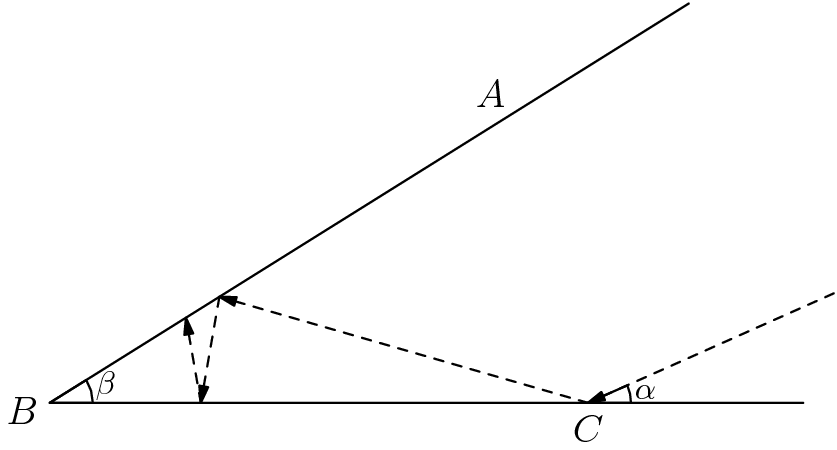
\includegraphics[width = 83.60000000000001mm]{img/fig0.png}
\end{center}